Using neural networks to learn (potentially high-dimensional) functions constrained by physical laws is a popular trend in scientific machine learning \cite{carleo2017solving, pfau2020ab, hermann2020deep, karniadakis2021physics, raissi2019physics, hu2023hutchinson, sun2020global}.
Typically, the Physics is encoded through partial differential equations (PDEs) that the neural net must satisfy.
The associated loss functions require evaluating differential operators \wrt the network's input, rather than weights.
Typically, evaluating the differential operator is a bottleneck since it contains higher-order derivatives.

\paragraph{Differential operators in the wild.} Two important fields of application are variational Monte-Carlo (VMC) and Physics-informed neural networks (PINNs).
VMC employs neural networks as ansatz for the Schr\"odinger equation \cite{carleo2017solving, pfau2020ab, hermann2020deep} and demands computing the net's Laplacian (the Hessian trace) to capture the kinetic energy in the Hamiltonian.
PINNs also use a neural net ansatz to learn a PDE solution and cast the problem as optimization task by minimizing the residuals of the governing equations \cite{raissi2019physics, karniadakis2021physics}.
This approach necessitates differentiable application of potentially high-order PDE operators.
For instance, the PINN formulation of Kolmogorov-type equations—including the Fokker-Planck, Black-Scholes, and Hamilton-Jacobi-Bellman equations—requires the evaluation of weighted second-order derivatives for high-dimensional spatial domains \cite{hu2023hutchinson, sun2024dynamical}.
The Biharmonic Operator occurs in PINNs for elasticity theory \cite{vahab_physics-informed_2022} and requires fourth-order derivatives of \wrt to the net's input. Due to the computational challenges associated with the fourth-order derivatives, the Biharmonic operator is commonly considered a benchmarking problem for PINNs \cite{hu2023hutchinson, vikas_biharm, shi2024stochastic}.

\paragraph{Is backpropagation all we need?}
% Alternative: The gap between theory and practise
Although it is known---at least on paper---that nesting first-order automatic differentiation (AD) to compute high-order derivatives scales poorly, this approach is common practise.
\todo{Felix: We should back this up with a reference, and optionally a statement about the scaling. I think the STDE paper does some analysis.}
The AD community has developed a more favourable alternative to nested backpropagation that promises faster computation of higher-order derivatives: \emph{Taylor-mode AD}~\cite[or simply \emph{Taylor-mode},][\S13]{griewank2008evaluating}.
\citet{bettencourt2019taylor} introduced Taylor-mode to the machine learning community in \citeyear{bettencourt2019taylor} and provided an implementation in JAX \cite{bradbury2018jax}.
However, we observe empirically that vanilla Taylor-mode is often not enough to beat nested backpropagation: We took a 5-layer $\tanh$ activated MLP (such nets are commonly used as PINNs) and evaluated its Laplacian using JAX's Taylor mode and compared its performance to computing, then tracing, the Hessian via Hessian-vector products \cite{pearlmutter1994fast,dagreou2024how}.
On this example, we found that \emph{vanilla Taylor mode is 50\% slower than nested backpropagation}.
This calls into question the relevance of Taylor mode for computing differential operators that ML practitioners are interested in.

\paragraph{No.}
\todo{Felix: Tone down, this is too much.}
Although it looks like, at first sight, backpropagation is all we need, recent works have successfully demonstrated the potential of Taylor mode and forward propagation schemes.
For the Laplacian, \citet{li2023forward} developed a special forward propagation framework called the \emph{forward Laplacian} (later generalized to weighted Laplacians \cite{li2024dof}).
Coming back to our example from above, we can see that JAX's forward Laplacian \cite{gao2023folx} outperforms nested backpropagation and is roughly twice as fast.
To stochastically approximate differential operators over extremely high-dimensional domains, \citet{shi2024stochastic} proposed using Taylor mode with carefully chosen randomly sampled directions.
While the forward Laplacian does not rely on Taylor mode, recent work pointed out a connection \cite{dangel2024kroneckerfactored}; however, it remains unclear what disentangles them, and if efficient forward schemes can also be derived for other differential operators.
Our work changes this.
We make the following contributions:
\todo{Felix: Make it more explicit that we evaluate Taylor mode in multiple directions and then sum the results. The sum can be pulled inside.}

\begin{figure*}[!t]
  \centering
  \begin{minipage}[b]{0.42\linewidth}
    \centering
    \input{figures/vanilla_taylor_not_enough.tex}

    \caption{\textbf{$\blacktriangle$ Vanilla Taylor mode is not enough to beat nested 1\textsuperscript{st}-order AD.}
      Illustrated for computing the Laplacian of a $\mathrm{tanh}$-activated $50 \!\to\! 768 \!\to\! 768 \!\to\! 512 \!\to\! 512 \!\to\! 1$
      MLP with JAX (+ \texttt{jit}) on GPU (details in \Cref{sec:jax-benchmark}).
      We show how to automatically obtain the specialized forward Laplacian through simple graph transformations of vanilla Taylor mode.
    }\label{fig:vanilla-taylor-not-enough}

    \vspace{0.25ex}
    \caption{\textbf{$\blacktriangleright$ Our collapsed Taylor mode directly propagates the sum of highest degree coefficients.}
      Visualized for propagating four $K$-jets through a $\sR^5 \!\to\! \sR^3 \!\to\! \sR$ function ($K=2$ yields the forward Laplacian).
      \Cref{sec:introduction} introduces the notation.}\label{fig:visual-abstract}
  \end{minipage}
  \hfill
  \begin{minipage}[b]{0.57\linewidth}
    \centering
    \newcommand{\drawgridrectangle}[4]{%
  \begin{tikzpicture}[scale=#4]
    \pgfmathsetmacro{\ymax}{#1}
    \pgfmathsetmacro{\xmax}{#2}

    % Fill the rectangle
    \fill[#3] (0,0) rectangle (\xmax,\ymax);

    % Draw the border
    \draw[white, line width=#4*3pt] (0,0) rectangle (\xmax,\ymax);


    % Draw vertical grid lines
    \pgfmathsetmacro{\xsteps}{#2}
    \foreach \x in {1,...,\xsteps} {
      \draw[white, line width=#4*3pt] (\x,0) -- (\x,\ymax);
    }

    % Draw horizontal grid lines
    \pgfmathsetmacro{\ysteps}{#1}
    \foreach \y in {1,...,\ysteps} {
      \draw[white, line width=#4*3pt] (0,\y) -- (\xmax,\y);
    }
  \end{tikzpicture}%
}

\newsavebox{\taylorStandard}
\savebox{\taylorStandard}{
  \begin{tikzpicture}
    \matrix [%
    matrix of nodes,%
    ampersand replacement=\&,% to use inside a savebox
    nodes={anchor=center, align=center},%
    column sep=4ex,%
    row sep=1ex,%
    ] (taylor)
    {
      \drawgridrectangle{1}{3}{blue!30}{0.33} \& \drawgridrectangle{1}{2}{blue!30}{0.33} \& \drawgridrectangle{1}{1}{blue!30}{0.33}
      \\[-1.5ex]
      $\vx_0$ \& $\vh_0$ \& $\vg_0$
      \\
      \drawgridrectangle{3}{3}{green!30}{0.33} \& \drawgridrectangle{3}{2}{green!30}{0.33} \& \drawgridrectangle{3}{3}{green!30}{0.33}
      \\[-1.5ex]
      $\{\vx_{1,d}\}$ \& $\{\vh_{1,d}\}$ \& $\{\vg_{1,d}\}$
      \\
      \drawgridrectangle{3}{3}{red!30}{0.33} \& \drawgridrectangle{3}{2}{red!30}{0.33} \& \drawgridrectangle{3}{1}{red!30}{0.33} \& \drawgridrectangle{1}{1}{red!60}{0.33}
      \\[-1.5ex]
      $\{\vx_{2,d}\}$ \& $\{\vh_{2,d}\}$ \& $\{\vg_{2,d}\}$ \& $\sum_d \vg_{2,d}$
      \\
    };

    % draw dependencies
    \pgfmathsetmacro{\K}{3}
    \pgfmathsetmacro{\L}{2}

    \foreach \l in {1,...,\L}{
      \pgfmathsetmacro{\lother}{int(\l+1)}
      \foreach \k in {1,...,\K} {
        \pgfmathsetmacro{\row}{int(2*\k-1)}
        \foreach \kother in {\k,...,\K} {
          \pgfmathsetmacro{\rowother}{int(2*\kother-1)}
          \draw[-Stealth, line width=1pt, white!50!black] (taylor-\row-\l.east) -- (taylor-\rowother-\lother.west);
        }
      }
    }
    \pgfmathsetmacro{\Lstart}{int(\L + 1)}
    \pgfmathsetmacro{\Lend}{int(\L + 2)}
    \pgfmathsetmacro{\rowfinal}{int(2*\K - 1)}
    \draw[-Stealth, line width=1pt, white!50!black] (taylor-\rowfinal-\Lstart.east) -- (taylor-\rowfinal-\Lend.west);
  \end{tikzpicture}
}

\newsavebox{\taylorCollapsed}
\savebox{\taylorCollapsed}{
  \begin{tikzpicture}
    \matrix [%
    matrix of nodes,%
    ampersand replacement=\&,% to use inside a savebox
    nodes={anchor=center, align=center},%
    column sep=4ex,%
    row sep=1ex,%
    ] (taylor)
    {
      \drawgridrectangle{1}{3}{blue!30}{0.33} \& \drawgridrectangle{1}{2}{blue!30}{0.33} \& \drawgridrectangle{1}{1}{blue!30}{0.33}
      \\[-1.5ex]
      $\vx_0$ \& $\vh_0$ \& $\vg_0$
      \\
      \drawgridrectangle{3}{3}{green!30}{0.33} \& \drawgridrectangle{3}{2}{green!30}{0.33} \& \drawgridrectangle{3}{3}{green!30}{0.33}
      \\[-1.5ex]
      $\{\vx_{1,d}\}$ \& $\{\vh_{1,d}\}$ \& $\{\vg_{1,d}\}$
      \\[2ex]
      \drawgridrectangle{1}{3}{red!60}{0.33} \& \drawgridrectangle{1}{2}{red!60}{0.33} \& \drawgridrectangle{1}{1}{red!60}{0.33}
      \\[-1.5ex]
      $\sum_d \vx_{2,d}$ \& $\sum_d \vh_{2,d}$ \& $\sum_d \vg_{2,d}$
      \\[1.1ex]
      \& \&
      \\
    };

    % draw dependencies
    \pgfmathsetmacro{\K}{3}
    \pgfmathsetmacro{\L}{2}

    \foreach \l in {1,...,\L}{
      \pgfmathsetmacro{\lother}{int(\l+1)}
      \foreach \k in {1,...,\K} {
        \pgfmathsetmacro{\row}{int(2*\k-1)}
        \foreach \kother in {\k,...,\K} {
          \pgfmathsetmacro{\rowother}{int(2*\kother-1)}
          \draw[-Stealth, line width=1pt, white!50!black] (taylor-\row-\l.east) -- (taylor-\rowother-\lother.west);
        }
      }
    }
  \end{tikzpicture}
}

\begin{figure*}[!t]
  \centering
  \resizebox{\linewidth}{!}{%
    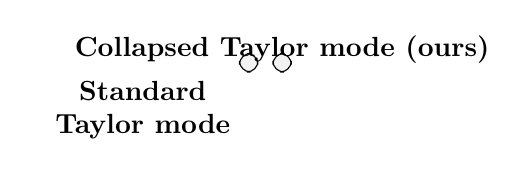
\begin{tikzpicture}
      \node (standard) [fill=black!5!white, draw=black, rounded corners]{\usebox{\taylorStandard}};
      \node [anchor=north east, align=center, inner sep=10pt] at (standard.north east) {\textbf{Standard} \\ \textbf{Taylor mode}};
      \node (collapsed) [fill=black!5!white, draw=black, rounded corners, anchor=north west, xshift=5pt] at (standard.north east) {\usebox{\taylorCollapsed}};
      \node [anchor=south, align=center, inner sep=3pt] at (collapsed.south) {\textbf{Collapsed Taylor mode (ours)}};
    \end{tikzpicture}
  }
  \caption{\textbf{Visual comparison of standard Taylor mode and our proposed collapsed Taylor mode.}}\label{fig:comparison-standard-vs-collapsed}
\end{figure*}

\begin{figure*}
  \centering
  \newsavebox{\taylorStandardNew}
  \savebox{\taylorStandardNew}{
    \begin{tikzpicture}
      \matrix [%
      matrix of nodes,%
      ampersand replacement=\&,% to use inside a savebox
      nodes={anchor=center, align=center},%
      column sep=5ex,%
      row sep=1ex,%
      ] (taylor)
      {
        \drawgridrectangle{1}{5}{gray!25!white}{0.33}
        \& \drawgridrectangle{1}{3}{gray!25!white}{0.33}
        \& \drawgridrectangle{1}{1}{gray!25!white}{0.33}
        \\[-1.5ex]
        $\vx_0$ \& $\vh_0$ \& $\vg_0$
        \\
        \drawgridrectangle{4}{5}{gray!50!white}{0.33}
        \& \drawgridrectangle{4}{3}{gray!50!white}{0.33}
        \& \drawgridrectangle{4}{1}{gray!50!white}{0.33}
        \\[-1.5ex]
        $\{\vx_{1,d}\}$ \& $\{\vh_{1,d}\}$ \& $\{\vg_{1,d}\}$
        \\[0.5ex]
        \drawgridrectangle{1}{5}{white}{0.33}
        \& \drawgridrectangle{1}{3}{white}{0.33}
        \& \drawgridrectangle{1}{1}{white}{0.33}
        \\[0.5ex]
        \\
        \drawgridrectangle{4}{5}{gray}{0.33}
        \& \drawgridrectangle{4}{3}{gray}{0.33}
        \& \drawgridrectangle{4}{1}{gray}{0.33}
        \\[-1.5ex]
        $\{\vx_{K-1,d}\}$ \& $\{\vh_{K-1,d}\}$ \& $\{\vg_{K-1,d}\}$
        \\[0.5ex]
        \drawgridrectangle{4}{5}{red!50}{0.33}
        \&
        \drawgridrectangle{4}{3}{red!50}{0.33}
        \&
        \drawgridrectangle{4}{1}{red!50}{0.33}
        \\[-1.5ex]
        $\{\vx_{K,d}\}$ \& $\{\vh_{K,d}\}$ \& $\{\vg_{K,d}\}$
        \\[-1.5ex]
        \textcolor{purple!50!red}{$\sum_d \vx_{K,d}$}
        \& \textcolor{purple!50!red}{$\sum_d \vh_{K,d}$}
        \& \textcolor{purple!50!red}{$\sum_d \vg_{K,d}$}
        \\
      };

      \node[xshift=-1pt, yshift=-14pt] at (taylor-9-1) {\drawgridrectangle{1}{5}{purple!50!red}{0.33}};
      \node[xshift=-1pt, yshift=-14pt] at (taylor-9-2) {\drawgridrectangle{1}{3}{purple!50!red}{0.33}};
      \node[xshift=-1pt, yshift=-14pt] at (taylor-9-3) {\drawgridrectangle{1}{1}{purple!50!red}{0.33}};

      \node at (taylor-5-1) {\vdots};
      \node at (taylor-5-2) {\vdots};
      \node at (taylor-5-3) {\vdots};

      % draw dependencies
      \pgfmathsetmacro{\K}{5}
      \pgfmathsetmacro{\L}{2}

      \foreach \l in {1,...,\L}{
        \pgfmathsetmacro{\lother}{int(\l+1)}
        \foreach \k in {1,...,\K} {
          \pgfmathsetmacro{\row}{int(2*\k-1)}
          \foreach \kother in {\k,...,\K} {
            \pgfmathsetmacro{\rowother}{int(2*\kother-1)}
            \draw[-Stealth, line width=1pt, gray] (taylor-\row-\l.east) -- (taylor-\rowother-\lother.west);
          }
        }
      }

      \coordinate (arrowStart) at ($(taylor-1-1.north)+(0,3.5ex)$);
      \coordinate (arrowEnd) at ($(taylor-1-3.north east)+(0,3.5ex)$);
      \draw[-Stealth, line width=2pt, black] (arrowStart) to node [midway, fill=white, align=center] {\textbf{Taylor forward} \\ \textbf{propagation}} (arrowEnd);

      \node [left=1.5ex of taylor-1-1] (zero) {0};
      \node [left=1.5ex of taylor-3-1] {1};
      \node [left=1.5ex of taylor-5-1] {$\vdots$};
      \node [left=1.5ex of taylor-7-1] {$K-1$};
      \node [left=1.5ex of taylor-9-1] {$K$};

      \node [align=center] (coefficientLabel) at ($(zero)+(0, 5.5ex)$) {\textbf{Derivative}\\\textbf{degree}};

      \draw[rounded corners] (taylor-9-1.north west) rectangle (taylor.south east);
    \end{tikzpicture}
  }

  \begin{tikzpicture}
    \node {\usebox{\taylorStandardNew}};
  \end{tikzpicture}
\end{figure*}

%%% Local Variables:
%%% mode: LaTeX
%%% TeX-master: "../main"
%%% End:

  \end{minipage}
\end{figure*}

\begin{enumerate}[leftmargin=0.5cm]
\item \textbf{We propose optimizing standard Taylor mode by collapsing the highest Taylor coefficients} and directly propagates their sum, rather than propagating then summing (\cref{fig:visual-abstract}).
  Collapsing standard Taylor mode for the Laplacian yields the forward Laplacian \cite{li2023forward}, but we show that this optimization is applicable to many other differential operators, and stochastic Taylor mode \cite{shi2024stochastic}.
  \todo{Felix: Phrase this so that it becomes clear that this is a theoretical contribution.}

\item \textbf{We show how to collapse standard Taylor mode by simple graph rewrites based on linearity.}
  This leads to a clean separation of concepts:
  Users can build their computational graph using standard Taylor mode, then use graph rewrites to collapse it.
  Due to the simple nature of our proposed rewrites, this feature could easily be absorbed into the just-in-time (JIT) compilation of ML frameworks, without introducing a new interface.

\item \textbf{We empirically demonstrate the performance improvements of collapsed Taylor mode.} Doing so, we introduce a Taylor mode library for PyTorch \cite{paszke2019pytorch}, realize the graph simplifications with \texttt{torch.fx} \cite{reed2022torch}, and show how that collapsing Taylor mode yields the theoretically expected improvements in run time and memory consumption.

\end{enumerate}

Our work takes an important step towards the broader adoption of Taylor mode as viable alternative to backpropagation for computing PDE operators, while being as easy to use. 

%%% Local Variables:
%%% mode: LaTeX
%%% TeX-master: "../main"
%%% End:
